\section{Linear Support Vector Classifier} \label{section:svc}

Given $n$ training points, where each input $x_i$ has $m$ attributes, i.e., is of dimensionality $m$, and is in one of two classes $y_i=\pm1$, i.e., our training data is of the form:

\begin{equation}
	\{(x_i,y_i), x_i\in\Re^m, y_i=\pm1, i=1, \dots, n\} \label{eq:svc_data}
\end{equation}

For simplicity we first assume that data are (not fully) linearly separable in the input space $x$, meaning that we can draw a line separating the two classes when $m=2$, a plane for $m=3$ and, more in general, a hyperplane for an arbitrary $m$.

Support vectors are the examples closest to the separating hyperplane and the aim of support vector machines is to orientate this hyperplane in such a way as to be as far as possible from the closest members of both classes, i.e., we need to maximize this margin.

This hyperplane is represented by the equation $w^T x + b=0$. So, we need to find $w$ and $b$ so that our training data can be described by:

\begin{equation} \label{eq:svc_consts}
	\begin{aligned}
		& w^T x_i + b \geq +1 - \xi_i, \forall y_i=+1 \\
    	& w^T x_i + b \leq -1 + \xi_i, \forall y_i=-1 \\
    	& \xi_i \geq 0 \ \forall_i
	\end{aligned}
\end{equation}

where the positive slack variables $\xi_i$ are introduced to allow misclassified points. In this way data points on the incorrect side of the margin boundary will have a penalty that increases with the distance from it.

These two equations can be combined into:

\begin{equation} \label{eq:svc_const}
	\begin{aligned}
    	& y_i (w^T x_i + b) \geq 1 - \xi_i \ \forall_i \\
    	& \xi_i\geq 0 \ \forall_i
    \end{aligned}
\end{equation}

The margin is equal to $\displaystyle \frac{1}{\| w \|}$ and maximizing it subject to the constraint in~\eqref{eq:svc_const} while as we are trying to reduce the number of misclassifications is equivalent to finding:

\begin{equation} \label{eq:svc_obj}
    \begin{aligned}
        \min_{w,b,\xi} \quad & \| w \| + C \sum_{i=1}^n \xi_i \\
            \text{subject to} \quad & y_i (w^T x_i + b) \geq 1 - \xi_i \ \forall_i \\ & \xi_i \geq 0 \ \forall_i
    \end{aligned}
\end{equation}

Minimizing $\| w \|$ is equivalent to minimizing $\displaystyle \frac{1}{2} \| w \|^2$, but in this form we will deal with a 1-strongly convex regularization term that has more desirable convergence properties. So we need to find:

\begin{equation} \label{eq:quad_svc_obj}
    \begin{aligned}
        \min_{w,b,\xi} \quad & \frac{1}{2} \| w \|^2 + C \sum_{i=1}^n \xi_i \\
            \text{subject to} \quad & y_i (w^T x_i + b) \geq 1 - \xi_i \ \forall_i \\ & \xi_i \geq 0 \ \forall_i
    \end{aligned}
\end{equation}

where the parameter $C$ controls the trade-off between the slack variable penalty and the size of the margin.

\begin{figure}[h!]
	\centering
	\includegraphics[scale=0.6]{img/linear_dual_svc_hyperplane}
	\caption{Linear SVC hyperplane}
	\label{fig:linear_dual_svc_hyperplane}
\end{figure}

\pagebreak

\subsection{Hinge loss}

The \emph{hinge} loss is defined as:

\begin{equation} \label{eq:hinge_loss1}
	\mathcal{L}_1 = \max(0, 1 - y (w^T x + b))
\end{equation}

or, equivalently:

\begin{equation} \label{eq:hinge_loss2}
	\mathcal{L}_1 = 
	\begin{cases}
		0 & \text{if} \ y (w^T x + b) \geq 1 \\
		1 - y (w^T x + b) & \text{otherwise} \\
	\end{cases}
\end{equation}

and it is a nondifferentiable convex function due to its nonsmoothness in 1, but has a subgradient that is given by:

\begin{equation} \label{eq:hinge_loss_der}
    \partial_w \mathcal{L}_1=
        \begin{cases}
            -y x & \text{if} \ y (w^T x + b) < 1 \\
            0 & \text{otherwise} \\ 
        \end{cases}
\end{equation}

\subsubsection{Primal formulation}

The general primal unconstrained formulation takes the form:

\begin{equation} \label{eq:primal_svm}
    \min_{w,b} \frac{1}{2} \| w \|^2 + C \sum_{i=1}^n \mathcal{L}(w,b;x_i,y_i)
\end{equation}

where $\displaystyle \frac{1}{2} \| w \|^2$ is the \emph{regularization term} and $\mathcal{L}(w,b;x_i,y_i)$ is the \emph{loss function} associated with the observation $(x_i,y_i)$~\cite{piccialli2018nonlinear}.

The quadratic optimization problem~\eqref{eq:quad_svc_obj} can be equivalently formulated as:

\begin{equation} \label{eq:primal_svc_hinge}
    \min_{w,b} \frac{1}{2} \| w \|^2 + C \sum_{i=1}^n \max(0, 1 - y_i (w^T x_i + b))
\end{equation}

where we make use of the \emph{hinge} loss~\eqref{eq:hinge_loss1} or~\eqref{eq:hinge_loss2}.

The above formulation penalizes slacks $\xi$ linearly and is called $\mathcal{L}_1$-SVC.

\begin{figure}[h!]
	\centering
  	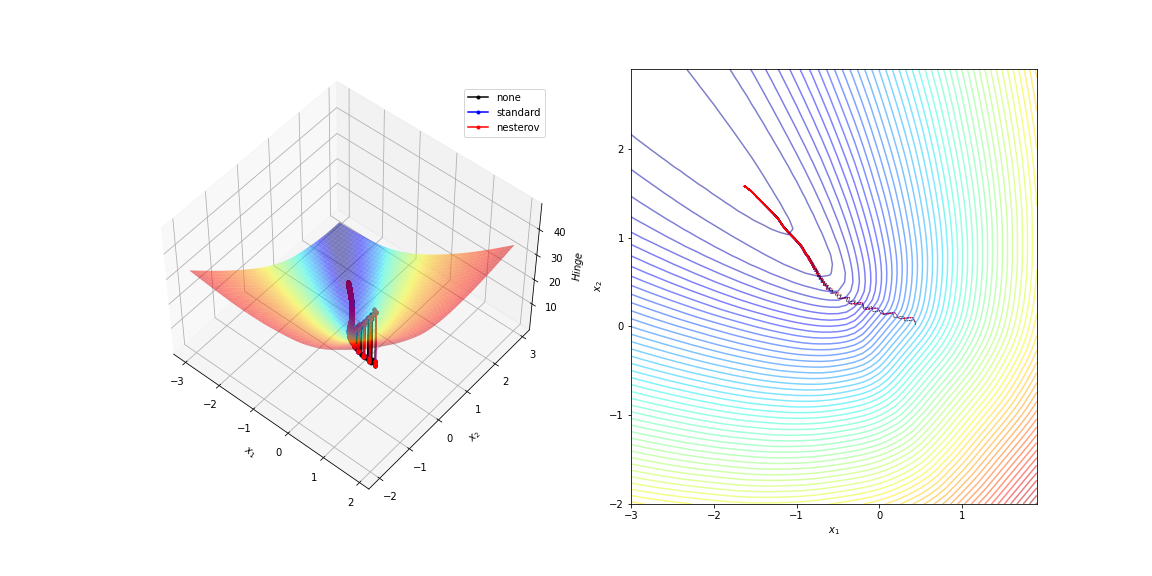
\includegraphics[scale=0.4]{img/svc_hinge_loss}
  	\caption{SVC Hinge loss with different optimization steps}
  	\label{fig:svc_hinge_loss}
\end{figure}

To simplify the notation and so also the design of the algorithms, the simplest approach to learn the bias term $b$ is that of including that into the \emph{regularization term}; so we can rewrite~\eqref{eq:primal_svm} as follows:

\begin{equation} \label{eq:biased_primal_svm1}
    \min_{w,b} \frac{1}{2} (\| w \|^2 + b^2) + C \sum_{i=1}^n \mathcal{L}(w,b;x_i,y_i)
\end{equation}

or, equivalently, by augmenting the weight vector $w$ with the bias term $b$ and each instance $x_i$ with an additional dimension, i.e., with constant value equal to 1:

\begin{equation} \label{eq:biased_primal_svm2}
    \begin{aligned}
        \min_{w} \quad & \frac{1}{2} \| \bar{w} \|^2 + C \sum_{i=1}^n \mathcal{L}(\bar{w};\bar{x}_i,y_i) \\
            \text{where} \quad & \bar{w}^T = [w^T, b] \\ & \bar{x}_i^T = [x_i^T, 1]
    \end{aligned}
\end{equation}

with the advantages of having convex properties of the objective function useful for convergence analysis and the possibility to directly apply algorithms designed for models without the bias term.

In the specific case of the $\mathcal{L}_1$-SVC the objective~\eqref{eq:primal_svc_hinge} become:

\begin{equation} \label{eq:biased_primal_svc_hinge}
    \min_{w,b} \frac{1}{2} (\| w \|^2 + b^2) + C \sum_{i=1}^n \max(0, 1 - y_i (w^T x_i + b))
\end{equation}

Notice that in terms of numerical optimization the formulation~\eqref{eq:primal_svc_hinge} is not equivalent to~\eqref{eq:biased_primal_svc_hinge} since in the first one the bias term $b$ does not contribute to the \emph{regularization term}, so the SVM formulation is based on an unregularized bias term $b$, as highlighted by the \emph{statistical learning theory}. But, in machine learning sense, numerical experiments in~\cite{hsu2002simple} show that the accuracy does not vary much when the bias term $b$ is embedded into the weight vector $w$.

\subsubsection{Wolfe Dual formulation}

To reformulate the~\eqref{eq:quad_svc_obj} as a \emph{Wolfe dual}, we need to allocate the Lagrange multipliers $\alpha_i\geq 0, \mu_i \geq 0 \ \forall_i$:

\begin{equation} \label{eq:svc_wolfe_dual}
    \max_{\alpha,\mu} \min_{w,b,\xi} \mathcal{W}(w,b,\xi,\alpha,\mu) = \frac{1}{2} \| w \|^2 + C \sum_{i=1}^n \xi_i-\sum_{i=1}^n \alpha_i(y_i(w^T x_i + b)-1+\xi_i)-\sum_{i=1}^n\mu_i\xi_i
\end{equation}

We wish to find the $w$, $b$ and $\xi_i$ which minimizes, and the $\alpha$ and $\mu$ which maximizes $\mathcal{W}$, provided $\alpha_i\geq 0, \mu_i \geq 0 \ \forall_i$. We can do this by differentiating $\mathcal{W}$ wrt $w$ and $b$ and setting the derivatives to 0:

\begin{equation} \label{eq:svc_wolfe_der_w}
	\frac{\partial \mathcal{W}}{\partial w}=w-\sum_{i=1}^n \alpha_i y_i x_i \Rightarrow w=\sum_{i=1}^n \alpha_i y_i x_i
\end{equation}

\begin{equation} \label{eq:svc_wolfe_der_b}
	\frac{\partial \mathcal{W}}{\partial b}=-\sum_{i=1}^n \alpha_i y_i\Rightarrow\sum_{i=1}^n \alpha_i y_i=0
\end{equation}

\begin{equation} \label{eq:svc_wolfe_der_xi}
	\frac{\partial \mathcal{W}}{\partial\xi_i}=0\Rightarrow C=\alpha_i+\mu_i
\end{equation}

Substituting~\eqref{eq:svc_wolfe_der_w} and~\eqref{eq:svc_wolfe_der_b} into~\eqref{eq:svc_wolfe_dual} together with $\mu_i\geq 0 \ \forall_i$, which implies that $\alpha\leq C$, gives a new formulation being dependent on $\alpha$. We therefore need to find:

\begin{equation} \label{eq:svc_max_wolfe_dual}
	\begin{aligned}
    	\max_{\alpha} \mathcal{W}(\alpha) &= \sum_{i=1}^n \alpha_i - \frac{1}{2}\sum_{i,j}\alpha_i\alpha_j y_i y_j \langle x_i, x_j \rangle \\
    	&= \sum_{i=1}^n \alpha_i - \frac{1}{2}\sum_{i,j}\alpha_i Q_{ij}\alpha_j \ \text{where} \ Q_{ij} = y_i y_j \langle x_i, x_j \rangle \\
    	&= \sum_{i=1}^n \alpha_i - \frac{1}{2}\alpha^T Q\alpha \ \text{subject to} \ 0\leq\alpha_i\leq C \ \forall_i, \sum_{i=1}^n \alpha_i y_i=0 
	\end{aligned}
\end{equation}

or, equivalently:

\begin{equation} \label{eq:svc_min_wolfe_dual}
    \begin{aligned}
        \min_{\alpha} \quad & \frac{1}{2}\alpha^T Q\alpha+q^T\alpha \\
            \text{subject to} \quad & 0\leq\alpha_i\leq C \ \forall_i \\ & y^T\alpha=0
    \end{aligned}
\end{equation}

where $q^T = [1, \dots, 1]$.

By solving~\eqref{eq:svc_min_wolfe_dual} we will know $\alpha$ and, from~\eqref{eq:svc_wolfe_der_w}, we will get $w$, so we need to calculate $b$.

We know that any data point satisfying~\eqref{eq:svc_wolfe_der_b} which is a support vector $x_s$ will have the form:

\begin{equation} \label{eq:svc_sv_const1}
	y_s(w^T x_s + b)=1
\end{equation}

and, by substituting in~\eqref{eq:svc_wolfe_der_w}, we get:

\begin{equation} \label{eq:svc_sv_const2}
	y_s\big(\sum_{m\in S}\alpha_m y_m \langle x_m, x_s \rangle +b\big)=1
\end{equation}

where $s$ denotes the set of indices of the support vectors and is determined by finding the indices $i$ where $\alpha_i>0$, i.e., nonzero Lagrange multipliers.

Multiplying through by $y_s$ and then using $y_s^2=1$ from~\eqref{eq:svc_consts}:

\begin{equation} \label{eq:svc_sv_squared_const2}
	y_s^2\big(\sum_{m\in S}\alpha_m y_m \langle x_m, x_s \rangle +b\big)=y_s
\end{equation}

\begin{equation} \label{eq:svc_b}
	b=y_s-\sum_{m\in S}\alpha_m y_m \langle x_m, x_s \rangle
\end{equation}

Instead of using an arbitrary support vector $x_s$, it is better to take an average over all of the support vectors in $S$:

\begin{equation} \label{eq:svc_b_avg}
	b=\frac{1}{N_s}\sum_{s\in S} y_s-\sum_{m\in S}\alpha_m y_m \langle x_m, x_s \rangle
\end{equation}

We now have the variables $w$ and $b$ that define our separating hyperplane's optimal orientation and hence our support vector machine. Each new point $x'$ is classified by evaluating:

\begin{equation} \label{eq:svc_pred}
    y'=\operatorname{sgn}\big(\sum_{i=1}^n\alpha_i y_i\langle x_i, x' \rangle+b\big)
\end{equation}

From~\eqref{eq:svc_min_wolfe_dual} we can notice that the equality constraint $y^T \alpha = 0$ arises form the stationarity condition $\partial_{{b}} \mathcal{W}=0$. So, again, for simplicity, we can again consider the bias term $b$ embedded into the weight vector. We report below the box-constrained dual formulation~\cite{hsu2002simple} that arises from the primal~\eqref{eq:biased_primal_svm1} or~\eqref{eq:biased_primal_svm2} where the bias term $b$ is embedded into the weight vector $w$:

\begin{equation} \label{eq:svc_min_bcqp_wolf_dual}
    \begin{aligned}
        \min_{\alpha} \quad & \frac{1}{2} \alpha^T (Q + yy^T)\alpha+q^T\alpha \\
            \text{subject to} \quad & 0\leq\alpha_i\leq C \ \forall_i
    \end{aligned}
\end{equation}

\subsubsection{Lagrangian Dual formulation}

In order to relax the constraints in the \emph{Wolfe dual} formulation~\eqref{eq:svc_min_wolfe_dual} we define the problem as a \emph{Lagrangian dual} relaxation by embedding them into objective function, so we need to allocate the Lagrangian multipliers $\mu \geq 0, \lambda_+ \geq 0$, $\lambda_- \geq 0$:

\begin{equation} \label{eq:svc_lagrangian_dual}
	\begin{aligned}
		    \max_{\mu,\lambda_+,\lambda_-} \min_{\alpha} \mathcal{L}(\alpha,\mu,\lambda_+,\lambda_-) &= \frac{1}{2} \alpha^T Q\alpha+q^T\alpha - \mu^T (y^T \alpha) - \lambda_+^T (u - \alpha) - \lambda_-^T \alpha \\
    &= \frac{1}{2} \alpha^T Q\alpha + (q - \mu y + \lambda_+ - \lambda_-)^T \alpha - \lambda_+^T u
	\end{aligned}
\end{equation}

where the upper bound $u^T = [C, \dots, C]$.

Taking the derivative of the Lagrangian $\mathcal{L}$ wrt $\alpha$ and settings it to 0 gives:

\begin{equation} \label{eq:svc_lagrangian_der_a}
	\frac{\partial \mathcal{L}}{\partial \alpha}=0\Rightarrow Q \alpha + (q - \mu y + \lambda_+ - \lambda_-) = 0
\end{equation}

With $\alpha$ optimal solution of the linear system:

\begin{equation} \label{eq:svc_lagrangian_sol}
    Q \alpha = - (q - \mu y + \lambda_+ - \lambda_-)
\end{equation}

the gradient wrt $\mu$, $\lambda_+$ and $\lambda_-$ are:

\begin{equation} \label{eq:svc_lagrangian_der_mu}
	\frac{\partial \mathcal{L}}{\partial \mu}=-y \alpha
\end{equation}

\begin{equation} \label{eq:svc_lagrangian_der_lp}
	\frac{\partial \mathcal{L}}{\partial \lambda_+}=\alpha - u
\end{equation}

\begin{equation} \label{eq:svc_lagrangian_der_lm}
    \frac{\partial \mathcal{L}}{\partial \lambda_-}=-\alpha
\end{equation}

From~\eqref{eq:svc_min_wolfe_dual} we can notice that the equality constraint $y^T \alpha = 0$ arises form the stationarity condition $\partial_{{b}} \mathcal{W}=0$. So, again, for simplicity, we can again consider the bias term $b$ embedded into the weight vector. In this way the dimensionality of~\eqref{eq:svc_lagrangian_dual} is reduced of 1/3 by removing the multipliers $\mu$ which was allocated to control the equality constraint $y^T \alpha=0$, so we will end up solving exactly the problem~\eqref{eq:svc_min_bcqp_wolf_dual}.

\begin{equation} \label{eq:svc_bcqp_lagrangian_dual}
	\begin{aligned}
    	\max_{\lambda_+,\lambda_-} \min_{\alpha} \mathcal{L}(\alpha,\lambda_+,\lambda_-) &= \frac{1}{2} \alpha^T (Q + yy^T)\alpha+q^T\alpha - \lambda_+^T (u - \alpha) - \lambda_-^T \alpha \\
    &= \frac{1}{2} \alpha^T (Q + yy^T)\alpha + (q + \lambda_+ - \lambda_-)^T \alpha - \lambda_+^T u
	\end{aligned}
\end{equation}

where, again, the upper bound $u^T = [C, \dots, C]$.

Now, taking the derivative of the Lagrangian $\mathcal{L}$ wrt $\alpha$ and settings it to 0 gives:

\begin{equation} \label{eq:svc_bcqp_lagrangian_der_a}
	\frac{\partial \mathcal{L}}{\partial \alpha}=0\Rightarrow (Q + yy^T) \alpha + (q + \lambda_+ - \lambda_-) = 0
\end{equation}

With $\alpha$ optimal solution of the linear system:

\begin{equation} \label{eq:svc_bcqp_lagrangian_sol}
    (Q + yy^T) \alpha = - (q + \lambda_+ - \lambda_-)
\end{equation}

the gradient wrt $\lambda_+$ and $\lambda_-$ are:

\begin{equation} \label{eq:svc_bcqp_lagrangian_der_lp}
	\frac{\partial \mathcal{L}}{\partial \lambda_+}=\alpha - u
\end{equation}

\begin{equation} \label{eq:svc_bcqp_lagrangian_der_lm}
    \frac{\partial \mathcal{L}}{\partial \lambda_-}=-\alpha
\end{equation}

\pagebreak

\subsection{Squared Hinge loss}

The \emph{squared hinge} loss is defined as:

\begin{equation} \label{eq:squared_hinge_loss2}
	\mathcal{L}_2 = \max(0, 1 - y (w^T x + b))^2
\end{equation}

or, equivalently:

\begin{equation} \label{eq:squared_hinge_loss1}
	\mathcal{L}_2 = 
	\begin{cases}
		0 & \text{if} \ y (w^T x + b) \geq 1 \\
		(1 - y (w^T x + b))^2 & \text{otherwise} \\
	\end{cases}
\end{equation}

It is a strictly convex function and its gradient is given by:

\begin{equation} \label{eq:squared_hinge_loss_der}
    \nabla_w \mathcal{L}_2=
        \begin{cases}
            - 2 y x & \text{if} \ y (w^T x + b) < 1 \\
            0 & \text{otherwise} \\ 
        \end{cases}
\end{equation}

\subsubsection{Primal formulation}

Since smoothed versions of objective functions may be preferred for optimization, we can reformulate~\eqref{eq:primal_svc_hinge} as:

\begin{equation} \label{eq:primal_svc_squared_hinge}
    \min_{w,b} \frac{1}{2} \| w \|^2 + C \sum_{i=1}^n \max(0, 1 - y_i (w^T x_i + b))^2
\end{equation}

where we make use of the \emph{squared hinge} loss that quadratically penalized slacks $\xi$ and is called $\mathcal{L}_2$-SVC.

The $\mathcal{L}_2$-SVC objective~\eqref{eq:primal_svc_squared_hinge} can be rewritten in form~\eqref{eq:biased_primal_svm1} or~\eqref{eq:biased_primal_svm2} as:

\begin{equation} \label{eq:biased_primal_svc_squared_hinge}
    \min_{w,b} \frac{1}{2} (\| w \|^2 + b^2) + C \sum_{i=1}^n \max(0, 1 - y_i (w^T x_i + b))^2
\end{equation}

\begin{figure}[h!]
	\centering
  	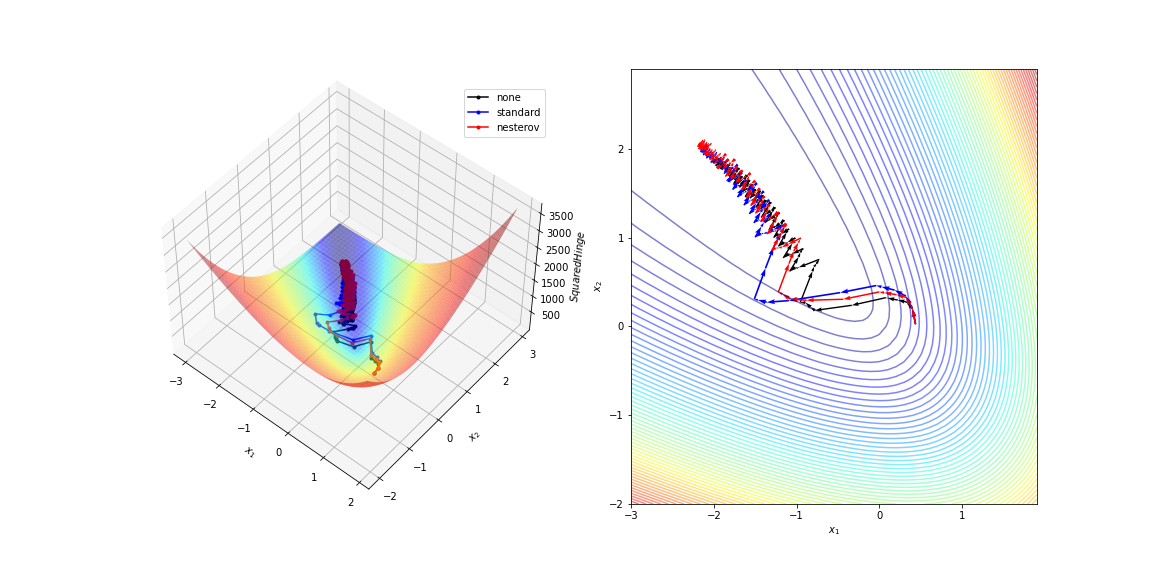
\includegraphics[scale=0.4]{img/svc_squared_hinge_loss}
  	\caption{SVC Squared Hinge loss with different optimization steps}
  	\label{fig:svc_squared_hinge_loss}
\end{figure}

\subsubsection{Wolfe Dual formulation}

As done for the $\mathcal{L}_1$-SVC we can derive the \emph{Wolfe dual} formulation of the $\mathcal{L}_2$-SVC by obtaining:

\begin{equation} \label{eq:wolfe_dual_svc_squared_hinge}
    \begin{aligned}
        \min_{\alpha} \quad & \frac{1}{2}\alpha^T (Q + D)\alpha+q^T\alpha \\
            \text{subject to} \quad & \alpha_i\geq 0 \ \forall_i \\ & y^T\alpha=0
    \end{aligned}
\end{equation}

or, alternatively, with the regularized bias term by obtaining:

\begin{equation} \label{eq:biased_wolfe_dual_svc_squared_hinge}
    \begin{aligned}
        \min_{\alpha} \quad & \frac{1}{2}\alpha^T (Q + yy^T + D) \alpha + q^T \alpha \\
            \text{subject to} \quad & \alpha_i \geq 0 \ \forall_i
    \end{aligned}
\end{equation}

where the diagonal matrix $\displaystyle D_{ii} = \frac{1}{2C} \ \forall_i$.

\subsubsection{Lagrangian Dual formulation}

In order to relax the constraints in the $\mathcal{L}_2$-SVC \emph{Wolfe dual} formulation~\eqref{eq:wolfe_dual_svc_squared_hinge} we define the problem as a \emph{Lagrangian dual} relaxation by embedding them into objective function, so we need to allocate the Lagrangian multipliers $\mu \geq 0, \lambda \geq 0$:

\begin{equation} \label{eq:l2_svc_lagrangian_dual}
	\begin{aligned}
		    \max_{\mu,\lambda} \min_{\alpha} \mathcal{L}(\alpha,\mu,\lambda) &= \frac{1}{2} \alpha^T (Q+D)\alpha+q^T\alpha - \mu^T (y^T \alpha) - \lambda^T \alpha \\
    &= \frac{1}{2} \alpha^T (Q+D)\alpha + (q - \mu y - \lambda)^T \alpha
	\end{aligned}
\end{equation}

Taking the derivative of the Lagrangian $\mathcal{L}$ wrt $\alpha$ and settings it to 0 gives:

\begin{equation} \label{eq:l2_svc_lagrangian_der_a}
	\frac{\partial \mathcal{L}}{\partial \alpha}=0\Rightarrow (Q+D) \alpha + (q - \mu y - \lambda) = 0
\end{equation}

With $\alpha$ optimal solution of the linear system:

\begin{equation} \label{eq:l2_svc_lagrangian_sol}
    (Q+D) \alpha = - (q - \mu y - \lambda)
\end{equation}

the gradient wrt $\mu$ and $\lambda$ are:

\begin{equation} \label{eq:l2_svc_lagrangian_der_mu}
	\frac{\partial \mathcal{L}}{\partial \mu}=-y \alpha
\end{equation}

\begin{equation} \label{eq:l2_svc_lagrangian_der_lambda}
    \frac{\partial \mathcal{L}}{\partial \lambda}=-\alpha
\end{equation}